In this section we introduce the computational metalanguage by example. We will
use the metalanguage to describe the semantics of a part of a simple generic instruction
set architecture. The later sections will introduce a formal definition of the
metalanguage, instruction and program semantics and present a method of extracting static
data dependencies of instructions with certain properties from the semantic definitions
leading to a construction of a~\emph{concurrent oracle}.

\begin{figure}[H]
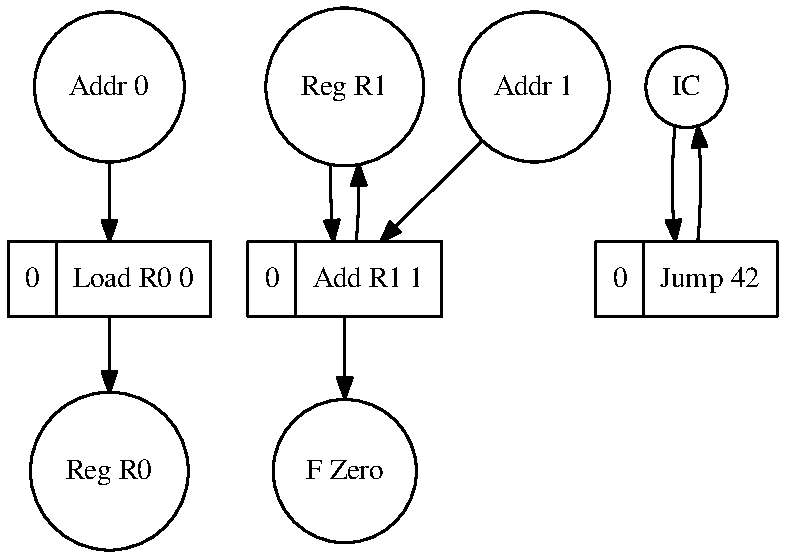
\includegraphics[width=35em]{img/loadJumpAdd.pdf}
\caption{Static data dependencies of~\hs{Load R0 0},~\hs{Add R1 1} and~\hs{Jump 42} instructions.}
\end{figure}

\subsubsection{Unconstrained semantics. Load} Literally every real-world instruction set include an instruction
which loads a data word from a memory location to a register. Here is how the
semantics of such an instruction can be encoded in the metalanguage:

\begin{minted}{haskell}
load reg addr = \read write -> Just $
    write (Reg reg) (read (Addr addr))
\end{minted}

In this definition we use two metalanguage terms:~\hs{read} and~\hs{write} to encode
the behaviour. These terms are polymorphic effectful functions with the following
types:

\begin{minted}{haskell}
read :: MachineKey -> f Word64
read =

write :: MachineKey -> f Word64 -> f ()
write =
\end{minted}

The~\hs{read} term queries the microarchitectural state for the value of a key and
returns it wrapped in a context~\hs{f}, which is, in fact, the reason for the
metalanguage to be~\emph{polymorphic}. In this case the context~\hs{f} may be any
type constructor of kind~\hs{* -> *}. However, not every instruction semantics may
be expressed in an unconstrained context. Let us consider semantics of some other
instructions to elaborate more on the nature of~\hs{f}.

\subsubsection{Functorial semantics. Jump}

Another popular instruction is the unconditional control flow transfer:

\begin{minted}{haskell}
jump offset = \read write -> Just $
    write IC ((+ offset) <$> (read IC))
\end{minted}

The semantics of this instruction increments the instruction counter~\hs{IC}
to transfer the control to another instruction in the program. This definition
has an crucial difference from~\hs{load}: it uses
the~\hs{<$>}\footnote{Function~\hs{<$>} (pronounced "fmap") of type
\hs{Functor f => (a -> b) -> f a -> f b} allows to transform the values in an
computational context with a pure function.} function of the~\hs{Functor} type
class, thus restricting~\hs{f} to be a~\hs{Functor}:

\begin{minted}{haskell}
read :: Functor f => MachineKey -> f Word64
read =

write :: Functor f => MachineKey -> f Word64 -> f ()
write =
\end{minted}

In this definition functorial constraint is required to apply the increment function
~\hs{(+ offset) :: Num a => a -> a} to the instruction counter enclosed in a computational
context~\hs{f}.

Later in the paper we will instantiate~\hs{f} as a context of data dependency
tracking. It turns out that the~\hs{Functor} constraint is equivalent to stating
that a computation may have at most one static dependency, being the instruction
counter in the case of~\hs{load}.

\subsubsection{Applicative semantics. Add}

The~\hs{add} instruction semantics performs the addition of the values of
a register and a memory cell. If the result of the addition is equal to zero,
the semantics sets the~\hs{Zero} microarchitectural flag~\hs{True}, or to~\hs{False} otherwise.

The Haskell definition of the semantic function is a bit more involved than the previous
ones. It turns out that the~\hs{Functor} context is not expressive enough and a
more powerful abstraction is needed. The following definition of~\hs{add} requires
\hs{f} to be at least an~\hs{Applicative}:

\begin{minted}{haskell}
add reg addr = \read write -> Just $
    let result = (+)    <$> read (Reg reg) <*> read (Addr addr)
        isZero = (== 0) <$> result
    in  write (Reg reg) result *>
        write (F Zero)  isZero
\end{minted}

Let us describe what is going on here. The definition may be broken down in three
classes of actions: reading data, processing it on-the-fly and writing data back in the store.

The first~\hs{let}-binding uses~\hs{Applicative} notation
to read the values from the register and memory address and add them up. Note that
this notation is~\emph{declarative}, hence it rather states that the~\hs{result}
is supposed to be a sum of values of two entities than performs actual computation.
This intuition is very important for understanding the static dependency tracking semantics
of instructions:~\hs{Reg reg} and~\hs{Addr addr} are declared as static input dependencies of
the~\hs{add} instruction. However, since the semantics may be executed in any~\hs{Applicative} context,
this dependency-tracking inspired intuition must not
obscure other possible interpretations of the semantics. For instance, in a stateful
simulation context, the~\hs{result} will be computed based on concrete data values
read from the underlying store.

The second line of the~\hs{let}-binding is quite similar to the expression in the
semantics of the~\hs{jump} instruction. The type of the~\hs{result} is~\hs{f Word64},
hence the zero testing function~\hs{(==) 0} of type~\hs{(Num a, Eq a) => a -> Bool}
must be mapped over the context~\hs{f} with~\hs{<$>} to obtain the value of type
\hs{f Bool}.

The latter two lines of the definition perform two~\hs{write} operations chained with
the applicative notation combinator~\hs{*>} of type~\hs{Applicative f => f a -> f b -> f b}.
This declares the values~\hs{Reg reg} and~\hs{F Zero} to be output dependencies of
the computation and that the writes mush be both performed.

An interesting feature of the~\hs{Applicative} notation is that it does not specify the exact order of
performing actions. This feature is useful in embedded domain-specific languages
with concurrency, for instance Facebook's Haxl~\cite{Marlow:2014:NFA:2692915.2628144}.

\hs{Applicative} functors are powerful enough to express the semantics of a
large class of instructions. In this paper we exploit their features to not only
specify the execution semantics but also automatically track static data dependencies
of instructions. However not every instruction of modern architecture may be
equipped with~\hs{Applicative} semantics. If the behaviour start to depend on the
actual data, i.e.~\emph{dynamic} data dependencies emerge, the semantics can not
be encoded using an~\hs{Applicative}. A more powerful abstraction is required.

\subsubsection{Monadic semantics. Memory indirect Load}

The indirect memory access instruction looks up a value in a memory cell and uses
it as the effective address in the regular load instruction. Since the effective
address can not be determined statically in the general case, this instruction
has a dynamic data dependency. The polymorphic computational metalanguage requires
the context~\hs{f} to be a~\hs{Monad} in order to be able to encode such behaviour.
Consider the definition of the semantics of the~\hs{loadMI} instruction, which
uses Haskell monadic ~\hs{do}-notation:

\begin{minted}{haskell}
loadMI reg addr read write = Just $ do
    addr' <- read (Addr addr)
    write (Reg reg) (read (Addr addr'))
\end{minted}

The first line extracts the effective address from the monadic context
and binds the identifier~\hs{addr'} to it. Here is the catch: expressions
on left-hand-side and right-hand-side of the~\hs{<-} symbol have different types.
The~\hs{read (Addr addr)} is of type~\hs{Monad f => f MemoryAddress} and the
identifier~\hs{addr'} has type \hs{MemoryAddress}. The main feature of~\hs{Monad}
is ability to extract a value from an effectful context and pass it in the further
computation as it was pure. This gives us a possibility to pass the~\hs{addr'}
as an argument to the next~\hs{read} operation.

Monadic semantics is more powerful that unconstrained, functorial and applicative ones,
but we are no more able to extract all the dependencies of the computation if
\hs{f} is restricted to~\hs{Monad}, since some of them will not be static. Therefore,
concurrency oracles can not be built for~\hs{Monad}-flavoured computations.

We have given examples of four kinds of semantic computations: unrestricted, functorial,
applicative and monadic. In every definition we used functions~\hs{read} and~\hs{write}
and have constrained the context~\hs{f} with~\hs{Functor},~\hs{Applicative}
or~\hs{Monad}. The resulting types of~\hs{read} and~\hs{write} follow a certain
pattern, which may be encoded in the Haskell type system. In fact, a generic
~\hs{read} may be assigned with type~\hs{forall c. MachineKey -> (c f) Word64} and
generic~\hs{write} with~\hs{forall c. MachineKey -> (c f) Word64 -> (c f) ()}. Here,
type variable~\hs{c} mush have kind~\hs{* -> Constraint}. This allows to instantiate
~\hs{c} with~\hs{Functor}, \hs{Applicative}, \hs{Monad} or any other suitable constraint,
thus making the metalanguage polymorphic in the computational context.

The next section will present a formal definition of the metalanguage, instruction
and program semantics. The section~\ref{oracles} will describe the construction of
concurrency oracles for programs comprising unrestricted, functorial, applicative,
but not monadic instructions.

